% Set the author and title of the compiled pdf
\hypersetup{
	pdftitle = {\Title},
	pdfauthor = {\Author}
}

\section{Keys and total orders}

It is often important to be able to implement some kind of comperator between
data items. This is often achieved in the from of a total order relation, which
has the following three properties:

\begin{description}
  \item \textbf{Reflexive property} 
    $k \leq k$
  \item \textbf{Antisymmetric property}
    $(k_1 \leq k_2 \wedge k_2 \leq k_1) \implies k_1 = k_2$
  \item \textbf{Transitive property} 
    $k_1 \leq k_2 \wedge k_2 \leq k_3 \implies k_1 \leq k_3$
\end{description}

A comperator that has the above three properties defines a linear ordering
relationship between data items. This means there will be a smallest item
$k_{min}$, where $k_{min} \leq K$ for all $K$ in the collections of data items.

\section{Trees}

\subsection{Definition}

A tree is an abstract data type for hierarchical storage of information. Each
element in a tree has a parent element, and zero or more children elements. The
node at the top of the tree is called the root.

A sub-tree is the tree consisting of all the descendents of a child of a tree,
including the child itself.

A tree is said to be \textit{ordered} if a linear ordering relation is defined
for the children of each node, that is to say that if we wanted to, we could
apply this relation to sort the children into an ordered list.

A binary tree is one where each node can have a maximum of two children. A
binary tree is \textit{proper} if each node as two (or zero) children. At each
level of a binary tree, the number of nodes in that level is at most $2^d$ where
$d$ is the level of the tree (starting from 0).

The depth of a node is the number of ancestors of the node excluding the node
itself.

% TODO: mention that recursive algorithms can be slooooowww for large trees
%       compared to an equivalent iterative algorithm. 

\subsection{Tree algorithms}

\subsubsection{Depth of a node}

The depth of a node in a tree is the number of ancestors of the node, excluding
the node itself.

\begin{javacode}
  int depth() {
    if(parent == null) { 
      // We've got no parent; we are the root!
      return 0;
    } else {
      return parent.depth() + 1;
    }
  }
\end{javacode}

This algorithm runs in $O(n)$ time and space, since it's dependent on the depth
of the tree, and is recursive.

\marginpar{Note that recursive algorithms always use space proportional to the
number of times they have recursed, since (unless tail recursion is used), each
recursion will use a stack frame.}

\subsection{Height of a tree}

A simple way to find the height of the tree, would be to iterate over every node
(maybe using a tree traversal algorithm mentioned in section~\ref{tree-
traversal}), and find the depth of each, keeping track of the maximum depth.
This would be a $O(n^2)$ algorithm.

A better approach is to use a recursive definition, and start from the root of
the tree. We can find the height of all of the child nodes, and return that plus
one.

\begin{javacode}
  int height() {
    if(children.size() == 0) return 0;
    else {
      int max = 0;
      for(Tree child : children) {
        int childHeight = child.height();
        if(childHeight > max) max = childHeight;
      }
      return max + 1;
    }
  }
\end{javacode}

\subsubsection{Tree traversal}

There are two different traversal schemes for trees; pre-order and post-order.
Each visits the elements in the tree in a different order. The following code
shows two different map functions, iterating in pre-order and then post order.

\begin{ccode}
  void mapPreOrder(Tree* root, void (*action)(Tree*)) {
    action(root);
    for(int i = 0; i < root->numChildren; i++) {
      root->children[i].mapInOrder(action);
    }
  }
  void mapPostOrder(Tree* root, void (*action)(Tree*)) {
    for(int i = 0; i < root->numChildren; i++) {
      root->children[i].mapInOrder(action);
    }
    action(root);
  }
\end{ccode}

You can also iterate in-order if your tree is a binary tree, you visit the left
child first, call the function on the current node, and then visit the right
child.

All the traversal algorithms take $O(n)$ time. 

\subsection{Tree datastructures}

There are two \textit{main} ways to store binary trees in memory; using a list
of nodes (in a heap style), or by using a linked datastructure, having nodes
point to other nodes.

\subsubsection{Using a vector based datastructure for trees}

In the vector (list/array/whatever you want to call it) style, the root of the
tree is stored at the start of the array. To calculate the index of the left
child of a node, you multiply the index of the current node by two. To find the
index of the right child of a node, you multiply its index by two and add one.
This numbering function is known as \textit{level numbering}, and can be
implemented like so:

\begin{ccode}
  int left(int n) { return 2 * n; }
  int right(int n) { return (2 * n) + 1; }
\end{ccode}

The running times of a vector-backed binary tree are good. Iteration can be done
in $O(n)$ time with a low overhead, swapping elements is $O(1)$ as is replacing
them.

\subsubsection{Using linked nodes to form a tree datastructure}

The trouble with using a vector datastructure, is you need to initialise an area
of memory equal to $2^{depth} \times sizeof(Tree)$. This means that for deep
trees, you will be wasting very large amounts of memory. This is a rather
extreme case of a memory-speed trade off.

In a linked data structure, each node points to all of its children. A really
simple example of a binary tree one could be:

\begin{javacode}
  public class Tree<T> {
    public Tree<T> left, right;
    public T value;
  }
\end{javacode}

If wanted to represent general (i.e. not binary) trees, we would have to modify
the datastructure so that we could have any number of children:

\begin{javacode}
  public class Tree<T> {
    public List<Tree<T>> children;
    public T value;
  }
\end{javacode}

\section{Priority Queues}

A priority queue is a datastructure capable of ordering items based on some
associated key. The two most important operations implemented on it are
\texttt{insertItem{priority, item}} and \texttt{removeMin()}.

Priority queues are the basis of some sorting algorithms, for example heap sort,
smooth sort, selection sort and insertion sort. The different type of sort
depends on how the priority queue is implemented. To sort a list using this
method, add all the items to the priority queue in any order, fill up the array
again in the order that the elements come out of the queue.

\begin{javacode}
  public <T implements Comparable<T>> List<T> sort(List<T> list) {
    PriorityQueue<T> pQueue = new PriotityQueue<T>();
    while(!list.isEmpty()) {
      pQueue.add(list.remove(0));
    }
    while(pQueue.isEmpty()) {
      list.add(pQueue.poll());
    }
    return list;
  }
\end{javacode}

\subsection{Heaps}

Priority queues are often implemented using a heap as the backing datastructure.
A heap is a binary tree that stores a collection of values. The type of values
stored by the heap must have a total order relationship, since otherwise, the
heap cannot be constructed correctly. The two properties that make heaps
different from normal binary trees are:

\begin{description}
  \item \textbf{Heap order property}:\\
    For every node $v$ in the tree, the value of $v$ is greater than or equal to
    the value of its parent. The only exception is the root, since that doesn't 
    have a parent.

    This means that if you start from the root, and move towards any leaf, then
    the nodes you encounter will be in a non-decreasing order. It also means 
    that the minimum key is at the root.
  \item \textbf{Complete binary tree property}:\\
    This means that if heap has a depth of $d$, then all levels of the tree from
    $0$ to $d-1$ must be completely full (i.e. they have $2^{level}$ nodes in),
    and the last level is filled up from left to right with the remaining
    elements.
\end{description}

There are no operations on a heap run that in worse than $O(log(n))$ time. The
operations are performed in a time proportional to the height of the tree rather
than the number of its elements.

\subsubsection{Insertion}

To store a new element in the heap, we add a new node to the heap at the next
available position (the last position in the tree). If the heap is backed by an
array, then the index of the array will be $n+1$, where $n$ is the current heap
size.

After we've inserted the new element we must check that the heap properties
aren't violated. The \textit{complete binary tree} property will be fine since
we added the element at the end of the array (which is always the last element
in the current level, or the first element in a new level), but the \textit{heap
order} property may be violated.

To maintain the \textit{heap order} property, we need to `bubble' the newly
inserted item up the heap until the property is restored. This is achieved by
comparing the key of the newly inserted node $n$ with its parent $p$. If $k(u)
> k(p)$, then they are swapped around (which is literally caused by indexes
the two items in the array). In the worst case, you would insert the (new)
smallest element into the heap, and the element would bubble all the way up to
the top, taking $log(n)$ time. This is called `up heap bubbling'.

\subsubsection{Removal}

If we want to remove the smallest element from the heap (as is required for a
priority queue), then that will be the root element of the heap. However, if we
just removed that element, then we would have two binary trees not one (a left
and a right tree).

Instead, we move the last element in the array into the first element, and
return the original first element (the last element is deleted). The
\textit{complete tree} property is now satisfied again. Now we have the element
previously at the bottom of the heap at the top, so we need to move it into a
position that will satisfy the  \textit{heap order} property.

To restore the \textit{heap order} property, we must `down heap bubble' the
root element. If the root element is the only node, then the property is
already satisfied. If the only child is on the left, then let $s$ be the left
child, and otherwise, let $s$ be the smallest (direct) child of the root node.

If $k(root) > k(s)$ then the heap order property is restored by swapping $r$
and $s$. You continue down the tree, swapping what was the route node until no
violation of the heap order property occurs. Since we may have to move all the
way down the tree from root to leaf, the runtime of this is also $O(log(n))$.

\subsubsection{Heap sort}

Since insertion and removal are both $O(log(n))$, and we're inserting $n$
elements, and then removing $n$ elements, then the runtime of a heap sort will
be $n \times n \log(n)$. Since constant factors are removed from the Big-O
notation, then the runtime is $O(n \log(n))$. This is a large improvement from
selection and insertion sort that take $n^2$ time. If the sequence was
implemented as an array, then the sort can be done in place too!

\section{Dictionaries and Hash Tables}

% This section is poorly explained

In a dictionary, the user assigns keys to elements, and the keys can be used to
look up elements in the datastructure (also known as a map in other languages
such as \texttt{java}). Dictionaries can be unordered, or ordered. When keys are
unique, then the dictionary is referred to as an associated store.

If the keys are unique, then a good way to implement the dictionary is a hash
table. Here, the key is hashed into an integer using a hashing function. The
result is used as the index of an array of `buckets'.

Each bucket stores a collection of values that have the same hashed key.
Ideally, each bucket will hold one element. This is easy to ensure for some
data, for example, if we had a Hash Table of the integers from 0-50, then we
could use the integer as the index to an array of fifty elements. In general
though, it is not possible to ensure that no collisions will occur, and one
bucket will probably end up with multiple elements. In this case, we need a
collision resolution strategy.

If we have a collision resolution strategy, then we don't need to have an array
that is as big as the number of items we're going to hold. We could just rely on
the collision resolution strategy to let us have a smaller array and therefore
need less contiguous memory space. Even if we do have the memory to spare, its
wasteful to have a massive array if we're only going to store a few items in
there.

If our hash function produces integers as indexes that are greater than the
number of buckets, then we can either take the modulus of that number by the
size of the array, or use the MAD method:

\[
  hash = |ak + b| mod N
\]

Where $N$ is a prime, and $a,b$ are random non-negative integers such that $a
mod N \neq 0$. The MAD (Multiply Add and Divide) method means the chance of a
collision is $\frac{1}{N}$.

\subsection{Collision handling}

There are different collision handling schemes, and each has its own benefits
and drawbacks. Here are just three:

\begin{description}
  \item \textbf{Separate chaining}:\\
    This is most often implemented using a Linked List for the buckets.
    Basically, when you want to add an item to the bucket, you just append it to
    the existing Linked List of items.
  \item \textbf{Open addressing}:\\
    In this strategy, if the index of the hash value is already occupied, then
    the buckets are examined in some sequence (the easiest is linear probing,
    which just looks at consecutive elements in the array), until a free slot
    is found.
  \item \textbf{Double hashing}:\\
    Here, a second hashing algorithm is used to find an alternative slot when 
    the first shows a collision. If we did $j$ attempts to find a new slot, the
    new index would be $hash1 + (j \times h(key))$, where $h$ is the second
    hashing algorithm.
\end{description}

Different collision resolution schemes exhibit different performance as the load
factor changes. The load factor is the number of entries divided by the number
of buckets.

If the load factor becomes too high, then we could \textit{rehash} the table.
This involves increasing the number of buckets, and re-inserting all the
elements currently in the table so that they are distributed according to the
new size of the array.

\subsubsection{Probing}

Probing is part of the open addressing collision resolution strategy. Linear
probing is easiest, you just walk through the array one by one until you find an
empty slot. Quadratic probing is harder, the next index to try and insert the
element into is found using an equation such as $|index + j^2| mod N$, where $j$
is the $j^{th}$ attempt at finding a slot.

Removing elements from a open addressed hash table is slightly more complicated,
but can be resolved by marking elements as `deactivated' rather than removing
them.

\section{Ordered Dictionaries}

An ordered dictionary is a key value store that lets you iterate over the keys
in order. This requirement means that we can't use a hash table to implement the
dictionary, so we need to use something else.

\subsection{Lookup tables}

We could order the keys with their associated values in a list by some
comperator and use the sorted nature of the keys to find the a specific pair. If
we were silly )or we'd chosen a linked list to implement the list), then we
would iterate through the whole array to find the pair we wanted. However, if we
were clever, then we could implement a binary search.

\subsubsection{Binary Search}

A binary search is an efficient way of searching though a sorted list for an
item. Basically, you start at index $\frac{n}{2}$, where $n$ is the number of
items in the list. If the index at that value is equal to the one you want, then
you've found the correct index! If its less than the one you want, then you
remove the bottom half of the list and start again, but if it's greater, then
you do the same for the top half of the list.

\begin{javacode}
  public static <T extends Comparable<T>> int binarySearch(T[] input, T item,
                                                           int start, int end) {
    if(start > end) return -1;
    else {
      int middleIndex = start + ((end - start) / 2);
      int comparison = item.compareTo(input[middleIndex]);
      if(comparison == 0) {
        return middleIndex;
      } else if(comparison < 0) {
        return binarySearch(input, item, start, middleIndex - 1);
      } else {
        return binarySearch(input, item, middleIndex + 1, end);
      }
    }
  }
\end{javacode}

Since we must do at most $log(n)$ recursions of the above algorithm (we halve
the input set every time), then the run time of the algorithm is $O(log(n))$.
Formally, this is because if $T(n)$ is the computational cost of a binary search
then:

\[
  T(n) = \begin{cases}
    c, & \text{if $n<2$}\\
    T(\frac{n}{2}) + c, & \text{Otherwise}
  \end{cases}
\]

\section{Binary Trees}

If you don't know what a binary tree is by this point in your degree then you
might not have been listening in all of your lectures, or in fact, reading my
notes properly.

You can use a binary tree as an ordered dictionary, since the keys can be stored
in the tree format, and they can each link to their respective values. The
runtime of a binary tree lookup is $O(n)$, as is insertion.

A perfectly balanced binary tree will exhibit a runtime of $O(log(n))$ for
search and insert, but maintaining a balanced binary tree requires extra effort.

\subsection{AVL Trees}

AVL trees are self balancing binary trees. The idea is that the datastructure
will re-order itself when it is mutated to stay close to the optimum shape. To
do this, we add an additional property onto that of the binary tree; the
\textit{height balance property}:

For every internal node $v$ of the tree $T$, the heights of its children can
differ by at most 1.

From this, we can derive the following properties about AVL trees:

\begin{itemize}
  \item Any subtree of an AVL tree is also an AVL tree itself.
  \item The height of an AVL tree that stores $n$ items is $O(log(n))$.
\end{itemize}

Since the maximum depth of an AVL tree is $log(n)$, searching for an item in the
tree is also an $O(log(n))$ operation.

\subsubsection{AVL tree insertion}

If our tree satisfies the height-balance property prior to us inserting a new
element, then after the element has been inserted, the heights of the nodes from
the root to the newly inserted node will increase by one. This could cause them
to violate the height-balance property.

To restore the balance to the tree, we use a strategy called \textit{search and
repair}:

\begin{itemize}
  \item Let $z$ by the first node on the path from the new node to the root that
    is unbalanced.
    \marginpar{See Figure~\ref{avl-tree-stage-1} for a description of where to
    put $z,y$ and $x$.}
  \item Denote $y$ to be the child of $z$ that has the larger height.
    \marginpar{Choose any ancestor of $z$ if there is a tie when choosing $y$
    or $x$.}
  \item Denote $x$ to be the child of $y$ that has the larger height.
  \item Since $z$ is unbalanced, we need to perform \textit{trinode
  restructuring}, which re-orders the tree but preserves the inorder traversal
  of the tree and runs in $O(1)$ time. There are four cases to this algorithm:
  \begin{description}
    \item \textbf{Left-left case}:\\
      \begin{verbatim}
       z                                      y 
      / \                                   /   \
     y   T4      Right Rotate (z)          x      z
    / \          - - - - - - - - ->      /  \    /  \ 
   x   T3                               T1  T2  T3  T4
  / \
T1   T2
      \end{verbatim}
    \item \textbf{Left-right case}:\\
      \begin{verbatim}
     z                               z                           x
    / \                            /   \                        /  \ 
   y   T4  Left Rotate (y)        x    T4  Right Rotate(z)    y      z
  / \      - - - - - - - - ->    /  \      - - - - - - - ->  / \    / \
T1   x                          y    T3                    T1  T2 T3  T4
    / \                        / \
  T2   T3                    T1   T2
      \end{verbatim}
    \item \textbf{Right-right case}:\\
      \begin{verbatim}
  z                                y
 /  \                            /   \ 
T1   y     Left Rotate(z)       z      x
    /  \   - - - - - - - ->    / \    / \
   T2   x                     T1  T2 T3  T4
       / \
     T3  T4
      \end{verbatim}
    \item \textbf{Right-left case}:\\
      \begin{verbatim}
   z                            z                            x
  / \                          / \                          /  \ 
T1   y   Right Rotate (y)    T1   x      Left Rotate(z)   z      y
    / \  - - - - - - - - ->     /  \   - - - - - - - ->  / \    / \
   x   T4                      T2   y                  T1  T2  T3  T4
  / \                              /  \
T2   T3                           T3   T4
      \end{verbatim}
  \end{description}
\end{itemize}

\begin{figure}[H]
  \centering
  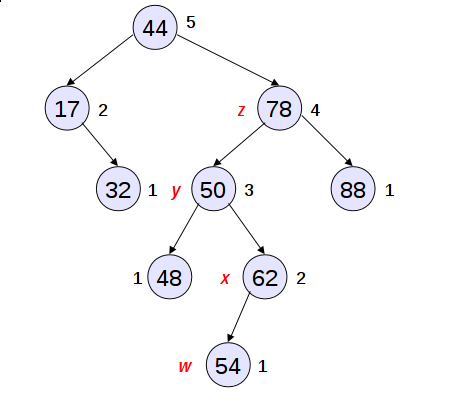
\includegraphics[width=0.5\textwidth]{images/avl-tree-stage-1}
  \caption{You can see the correct choices of $z$, $y$ and $x$ when searching an
  AVL tree after an insert}
  \label{avl-tree-stage-1}
\end{figure}

\subsubsection{AVL tree removal}

If we remove an external node, then the height balance property of the AVL tree
will remain satisfied, but if we remove an internal node, then it might not be.
In this case, the node is removed as normal, but we again apply the trinode
restructuring after its been removed to restore the balance.

Once you have applied the trinode restructuring once, you need to carry on
moving up the tree and checking the balance, since otherwise there could still
be unbalanced nodes higher up the tree. Since the maximum number of times we'll
need to restructure the tree is equal to the depth of the tree, removal is
$O(log(n))$.

\section{Problem solving}

Three techniques for implementing algorithms are looked at in this course;
divide-and-conquer, greedy strategies and dynamic programming.

\subsection{Divide and Conquer}

Divide and conquer is a design paradigm based on multi-branch recursion. This
means that at each stage of the problem, we split the problem into parts that
can be solved by the same algorithm. This has the effect of reducing the problem
into something smaller every time. Eventually, we will have reduced the input
set for any one problem into something much smaller, at which point it is
significantly easier to solve the problem (since the size of the input set is
small).

The divide and conquer technique is very popular, for example MergeSort, and
QuickSort are both based on it, you can do integer multiplication with it, and
even solve nearest neighbour problems (like the ones in \texttt{COMP24111}. You
can even use it for the last lab in this course (ex13) to split up the input set
of nodes into chunks and process them individually.

\subsubsection{D\&C Example}

Lets imagine we want to find the largest and smallest numbers in a set of
integers. We could do this in $O(n)$ very easily (see Figure~\ref{easy-soln}),
so the divide and conquer algorithm isn't really needed here, however, this
problem is still a good demonstration of the technique.

\begin{figure}[H]
  \label{easy-soln}
  \inputminted{java}{code/MinMax/Easy.java}
  \caption{Solving the largest/smallest integer problem is easy to do, even in
  $O(n)$ time.}
\end{figure}

To solve the problem using the Divide and Conquer strategy, we should split the
input list into two at the start of the method, and run the algorithm
recursively on the two sub-lists. Then, when the sublist length is either one or
two, a pair should be generated of the maximum and the minimum, which is then
returned. Once the method has two pairs of max/min elements from its sublists,
then it should combine them by finding the smallest and largest from the two
pairs. See Figure~\ref{d-and-c-soln} for a simple implementation.

\begin{figure}[H]
  \label{d-and-c-soln}
  \inputminted{java}{code/MinMax/DivideAndConquer.java}
  \caption{We can also solve the largest/smallest integer problem using divide
  and conquer.}
\end{figure}

While the run time of the Divide and Conquer solution may not be significantly
faster than the Easy one, there are other advantages, and disadvantages.
Obviously, the divide and conquer one uses more memory space, since we're using
recursion, we add a new frame onto the stack for every recursive call. However,
we could parallelise the divide and conquer solution much more easily (which can
bring near-linear performance gains).

\subsection{Greedy method}

The greedy method is a heuristic for making the optimal choice at each stage of
a problem. For example, if we wanted to give the correct change for $36p$, then
we would first choose the highest coin that fits into that, which is a $20p$,
and then choose the highest coin that fits into $36-20=16p$, which is $10p$, and
then the highest that fits into $16 - 10 = 6$, which is $5p$ and then $1p$,
since that's what we have left.

Since greedy is a heuristic, it doesn't always work optimally. For example, if
we had the coin values $10, 6$ and $1$ and were trying to make $12$, then greedy
would pick $10,1,1$, but the optimal solution is $6,6$.

\marginpar{An implementation of this is at the end of the document,
Figure~\ref{greedy}.}

For some applications, a greedy strategy is always successful, but for others,
it will perform poorly, or not find solutions at all. Greedy-applicable problems
include path finding, job scheduling, knapsack problems etc.

\subsection{Dynamic programming}

In general, the greedy method fails for the coin problem, and many other
problems too! Dynamic programming can always produce optimal solutions to some
of the problems that greedy will fail at.

Lets solve the coin problem with dynamic programming. To do this, we build up a
solution from the bottom and word towards a complete solution.

If we had the coins $9,1,5$ and $6$ and we were trying to make the number $11$,
then the greedy method would use $9,1,1$ as the coins. With dynamic programming,
we build up an array of sub-problem solutions and use those results to form
better solutions:

\begin{center}
  \begin{tabular}{c | c c c c c c c c c c c}
    Coins & 1 & 2 & 3 & 4 & 5 & 6 & 7 & 8 & 9 & 10 & 11\\ \hline
    $1$   & $\infty$ & $\infty$ & $\infty$ & $\infty$ & $\infty$ & $\infty$ & $\infty$ & $\infty$ & 1 & $\infty$ & $\infty$ \\
    $1,9$ & 1 & 2 & 3 & 4 & 5 & 6 & 7 & 8 & 1 & 2 & 3\\
    $1,9,5$ & 1 & 2 & 3 & 4 & 1 & 2 & 3 & 4 & 1 & 2 & 3\\
    $1,9,5,6$ & 1 & 2 & 3 & 4 & 1 & 1 & 2 & 3 & 1 & 2 & 2\\
  \end{tabular}
\end{center}

The efficiency of DP is the number of rows in the table multiplied by the number
of columns. Sometimes, you can save CPU time by not computing all of the
subproblems, but that might be problematic, since you could need them later.

Dynamic programming can be applied to path finding, text similarity tests,
knapsack problems etc.

\section{Misc figures}

These were too big to go in other places, so I shoved them at the end.

\begin{figure}[H]
  \label{greedy}
  \inputminted{java}{code/Greedy/Greedy.java}
  \caption{An implementation of the greedy money counter.}
\end{figure}

\subsection{Tractable and Intractable Problems}

Divide and Conquer and Greedy Strategies give us fast (polynomial time)
algorithms, and Dynamic Programming gives us fast algorithms, but also
algorithms that work on intractable problems.

A problem is considered tractable if we can produce a polynomial ($O(1), O(n),
O(n^x)$) time algorithm to solve it. Algorithms are intractable if they are
exponential, such as $O(2^n), O(n^n), O(n!)$.

Exponential algorithms often arise from exhaustive enumeration (i.e. checking
all the possible solutions), or systematic searches of partial solutions using
backtracking. If we wanted to colour a graph (that is give each node a colour,
but make sure that no adjacent nodes had the same colour), we could use both
techniques.

Exhaustive enumeration is the most simple approach to graph colouring; you start
with $k$ colours, and enumerate all the allocations of the colours on the nodes,
and for each, you check to see if its valid. Checking an allocation takes $O(E)$
time, \marginpar{$E$ is the number of edges, $N$ is the number of nodes.} but
there are $k^N$ number of allocations, so the algorithm takes $O(E \times k^N)$
time.
